\documentclass{standalone}
\usepackage{tikz}
\usetikzlibrary{patterns, positioning}

\begin{document}
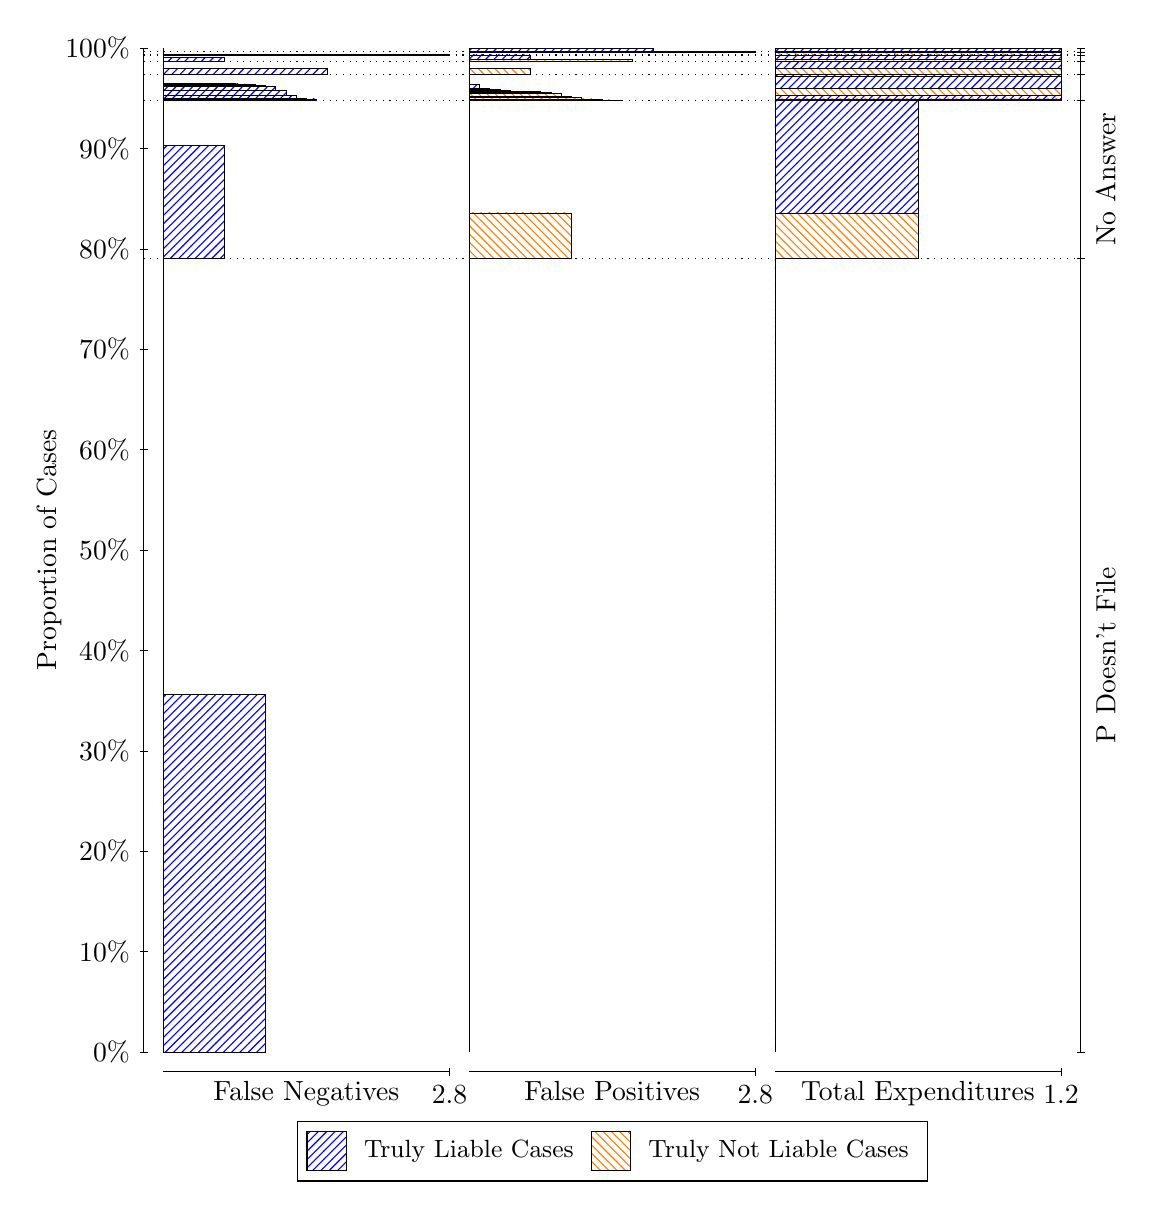
\begin{tikzpicture}
\draw[black, very thin] (1.5,1.75) -- (1.5,14.5);
\node[rotate=90, anchor=center] at (0.3, 8.125) {Proportion of Cases};
\draw[black, very thin] (1.45,1.75) -- (1.55,1.75);
\node[anchor=east] at (1.45, 1.75) {0\%};
\draw[black, very thin] (1.45,3.025) -- (1.55,3.025);
\node[anchor=east] at (1.45, 3.025) {10\%};
\draw[black, very thin] (1.45,4.3) -- (1.55,4.3);
\node[anchor=east] at (1.45, 4.3) {20\%};
\draw[black, very thin] (1.45,5.575) -- (1.55,5.575);
\node[anchor=east] at (1.45, 5.575) {30\%};
\draw[black, very thin] (1.45,6.85) -- (1.55,6.85);
\node[anchor=east] at (1.45, 6.85) {40\%};
\draw[black, very thin] (1.45,8.125) -- (1.55,8.125);
\node[anchor=east] at (1.45, 8.125) {50\%};
\draw[black, very thin] (1.45,9.4) -- (1.55,9.4);
\node[anchor=east] at (1.45, 9.4) {60\%};
\draw[black, very thin] (1.45,10.675) -- (1.55,10.675);
\node[anchor=east] at (1.45, 10.675) {70\%};
\draw[black, very thin] (1.45,11.95) -- (1.55,11.95);
\node[anchor=east] at (1.45, 11.95) {80\%};
\draw[black, very thin] (1.45,13.225) -- (1.55,13.225);
\node[anchor=east] at (1.45, 13.225) {90\%};
\draw[black, very thin] (1.45,14.5) -- (1.55,14.5);
\node[anchor=east] at (1.45, 14.5) {100\%};

\draw[black, very thin] (13.4,1.75) -- (13.4,14.5);
\draw[black, very thin] (13.35,1.75) -- (13.45,1.75);
\node[anchor=west] at (13.35, 1.75) {};
\draw[black, very thin] (13.35,11.831) -- (13.45,11.831);
\node[anchor=west] at (13.35, 11.831) {};
\draw[black, very thin] (13.35,13.837) -- (13.45,13.837);
\node[anchor=west] at (13.35, 13.837) {};
\draw[black, very thin] (13.35,14.161) -- (13.45,14.161);
\node[anchor=west] at (13.35, 14.161) {};
\draw[black, very thin] (13.35,14.326) -- (13.45,14.326);
\node[anchor=west] at (13.35, 14.326) {};
\draw[black, very thin] (13.35,14.412) -- (13.45,14.412);
\node[anchor=west] at (13.35, 14.412) {};
\draw[black, very thin] (13.35,14.451) -- (13.45,14.451);
\node[anchor=west] at (13.35, 14.451) {};
\draw[black, very thin] (13.35,14.5) -- (13.45,14.5);
\node[anchor=west] at (13.35, 14.5) {};

\draw[black, very thin, pattern color=blue, pattern=north east lines] (1.75,1.75) rectangle (3.0476,6.2927);
\draw[black, very thin, pattern color=orange, pattern=north west lines] (1.75,6.2927) rectangle (1.75,11.831);
\draw[black, very thin, pattern color=blue, pattern=north east lines] (1.75,11.831) rectangle (2.5286,13.262);
\draw[black, very thin, pattern color=orange, pattern=north west lines] (1.75,13.262) rectangle (1.75,13.837);
\draw[black, very thin, pattern color=blue, pattern=north east lines] (1.75,13.837) rectangle (3.6964,13.855);
\draw[black, very thin, pattern color=blue, pattern=north east lines] (1.75,13.855) rectangle (3.5667,13.862);
\draw[black, very thin, pattern color=blue, pattern=north east lines] (1.75,13.862) rectangle (3.4369,13.902);
\draw[black, very thin, pattern color=blue, pattern=north east lines] (1.75,13.902) rectangle (3.3071,13.964);
\draw[black, very thin, pattern color=blue, pattern=north east lines] (1.75,13.964) rectangle (3.1774,14.013);
\draw[black, very thin, pattern color=blue, pattern=north east lines] (1.75,14.013) rectangle (3.0476,14.029);
\draw[black, very thin, pattern color=blue, pattern=north east lines] (1.75,14.029) rectangle (2.9179,14.039);
\draw[black, very thin, pattern color=blue, pattern=north east lines] (1.75,14.039) rectangle (2.7881,14.044);
\draw[black, very thin, pattern color=blue, pattern=north east lines] (1.75,14.044) rectangle (2.6583,14.048);
\draw[black, very thin, pattern color=orange, pattern=north west lines] (1.75,14.048) rectangle (1.75,14.161);
\draw[black, very thin, pattern color=blue, pattern=north east lines] (1.75,14.161) rectangle (3.8262,14.243);
\draw[black, very thin, pattern color=orange, pattern=north west lines] (1.75,14.243) rectangle (1.75,14.326);
\draw[black, very thin, pattern color=blue, pattern=north east lines] (1.75,14.326) rectangle (2.5286,14.385);
\draw[black, very thin, pattern color=orange, pattern=north west lines] (1.75,14.385) rectangle (1.75,14.412);
\draw[black, very thin, pattern color=blue, pattern=north east lines] (1.75,14.412) rectangle (5.3833,14.421);
\draw[black, very thin, pattern color=orange, pattern=north west lines] (1.75,14.421) rectangle (1.75,14.451);
\draw[black, very thin, pattern color=orange, pattern=north west lines] (1.75,14.451) rectangle (1.75,14.46);
\draw[black, very thin, pattern color=blue, pattern=north east lines] (1.75,14.46) rectangle (1.75,14.5);
\draw[black, very thin, pattern color=orange, pattern=north west lines] (5.6333,1.75) rectangle (5.6333,7.2879);
\draw[black, very thin, pattern color=blue, pattern=north east lines] (5.6333,7.2879) rectangle (5.6333,11.831);
\draw[black, very thin, pattern color=orange, pattern=north west lines] (5.6333,11.831) rectangle (6.931,12.406);
\draw[black, very thin, pattern color=blue, pattern=north east lines] (5.6333,12.406) rectangle (5.6333,13.837);
\draw[black, very thin, pattern color=orange, pattern=north west lines] (5.6333,13.837) rectangle (7.5798,13.839);
\draw[black, very thin, pattern color=orange, pattern=north west lines] (5.6333,13.839) rectangle (7.45,13.842);
\draw[black, very thin, pattern color=orange, pattern=north west lines] (5.6333,13.842) rectangle (7.3202,13.847);
\draw[black, very thin, pattern color=orange, pattern=north west lines] (5.6333,13.847) rectangle (7.1905,13.855);
\draw[black, very thin, pattern color=orange, pattern=north west lines] (5.6333,13.855) rectangle (7.0607,13.871);
\draw[black, very thin, pattern color=orange, pattern=north west lines] (5.6333,13.871) rectangle (6.931,13.889);
\draw[black, very thin, pattern color=orange, pattern=north west lines] (5.6333,13.889) rectangle (6.8012,13.922);
\draw[black, very thin, pattern color=orange, pattern=north west lines] (5.6333,13.922) rectangle (6.6714,13.932);
\draw[black, very thin, pattern color=orange, pattern=north west lines] (5.6333,13.932) rectangle (6.5417,13.95);
\draw[black, very thin, pattern color=blue, pattern=north east lines] (5.6333,13.95) rectangle (6.2821,13.954);
\draw[black, very thin, pattern color=blue, pattern=north east lines] (5.6333,13.954) rectangle (6.1524,13.959);
\draw[black, very thin, pattern color=blue, pattern=north east lines] (5.6333,13.959) rectangle (6.0226,13.97);
\draw[black, very thin, pattern color=blue, pattern=north east lines] (5.6333,13.97) rectangle (5.8929,13.985);
\draw[black, very thin, pattern color=blue, pattern=north east lines] (5.6333,13.985) rectangle (5.7631,14.034);
\draw[black, very thin, pattern color=blue, pattern=north east lines] (5.6333,14.034) rectangle (5.6333,14.161);
\draw[black, very thin, pattern color=orange, pattern=north west lines] (5.6333,14.161) rectangle (6.4119,14.244);
\draw[black, very thin, pattern color=blue, pattern=north east lines] (5.6333,14.244) rectangle (5.6333,14.326);
\draw[black, very thin, pattern color=orange, pattern=north west lines] (5.6333,14.326) rectangle (7.7095,14.353);
\draw[black, very thin, pattern color=blue, pattern=north east lines] (5.6333,14.353) rectangle (6.4119,14.412);
\draw[black, very thin, pattern color=orange, pattern=north west lines] (5.6333,14.412) rectangle (5.6333,14.441);
\draw[black, very thin, pattern color=blue, pattern=north east lines] (5.6333,14.441) rectangle (5.6333,14.451);
\draw[black, very thin, pattern color=orange, pattern=north west lines] (5.6333,14.451) rectangle (9.2667,14.46);
\draw[black, very thin, pattern color=blue, pattern=north east lines] (5.6333,14.46) rectangle (7.969,14.5);
\draw[black, very thin, pattern color=orange, pattern=north west lines] (9.5167,1.75) rectangle (9.5167,7.2879);
\draw[black, very thin, pattern color=blue, pattern=north east lines] (9.5167,7.2879) rectangle (9.5167,11.831);
\draw[black, very thin, pattern color=orange, pattern=north west lines] (9.5167,11.831) rectangle (11.333,12.406);
\draw[black, very thin, pattern color=blue, pattern=north east lines] (9.5167,12.406) rectangle (11.333,13.837);
\draw[black, very thin, pattern color=orange, pattern=north west lines] (9.5167,13.837) rectangle (13.15,13.853);
\draw[black, very thin, pattern color=blue, pattern=north east lines] (9.5167,13.853) rectangle (13.15,13.902);
\draw[black, very thin, pattern color=orange, pattern=north west lines] (9.5167,13.902) rectangle (13.15,13.992);
\draw[black, very thin, pattern color=blue, pattern=north east lines] (9.5167,13.992) rectangle (13.15,14.138);
\draw[black, very thin, pattern color=orange, pattern=north west lines] (9.5167,14.138) rectangle (13.15,14.146);
\draw[black, very thin, pattern color=blue, pattern=north east lines] (9.5167,14.146) rectangle (13.15,14.161);
\draw[black, very thin, pattern color=orange, pattern=north west lines] (9.5167,14.161) rectangle (13.15,14.244);
\draw[black, very thin, pattern color=blue, pattern=north east lines] (9.5167,14.244) rectangle (13.15,14.326);
\draw[black, very thin, pattern color=orange, pattern=north west lines] (9.5167,14.326) rectangle (13.15,14.353);
\draw[black, very thin, pattern color=blue, pattern=north east lines] (9.5167,14.353) rectangle (13.15,14.412);
\draw[black, very thin, pattern color=orange, pattern=north west lines] (9.5167,14.412) rectangle (13.15,14.441);
\draw[black, very thin, pattern color=blue, pattern=north east lines] (9.5167,14.441) rectangle (13.15,14.451);
\draw[black, very thin, pattern color=orange, pattern=north west lines] (9.5167,14.451) rectangle (13.15,14.46);
\draw[black, very thin, pattern color=blue, pattern=north east lines] (9.5167,14.46) rectangle (13.15,14.5);
\draw[black, dotted] (1.5,11.831) -- (13.4,11.831);
\draw[black, dotted] (1.5,13.837) -- (13.4,13.837);
\draw[black, dotted] (1.5,14.161) -- (13.4,14.161);
\draw[black, dotted] (1.5,14.326) -- (13.4,14.326);
\draw[black, dotted] (1.5,14.412) -- (13.4,14.412);
\draw[black, dotted] (1.5,14.451) -- (13.4,14.451);
\draw[black, very thin] (1.75,1.5) -- (5.3833,1.5);
\node[anchor=north] at (3.5667, 1.5) {False Negatives};
\draw[black, very thin] (5.3833,1.45) -- (5.3833,1.55);
\node[anchor=north] at (5.3833, 1.45) {2.8};

\draw[black, very thin] (5.6333,1.5) -- (9.2667,1.5);
\node[anchor=north] at (7.45, 1.5) {False Positives};
\draw[black, very thin] (9.2667,1.45) -- (9.2667,1.55);
\node[anchor=north] at (9.2667, 1.45) {2.8};

\draw[black, very thin] (9.5167,1.5) -- (13.15,1.5);
\node[anchor=north] at (11.333, 1.5) {Total Expenditures};
\draw[black, very thin] (13.15,1.45) -- (13.15,1.55);
\node[anchor=north] at (13.15, 1.45) {1.2};

\node[black, centered, rotate=90] at (13.72, 6.7903) {P Doesn't File};
\node[black, centered, rotate=90] at (13.72, 12.834) {No Answer};






\draw (7.449999999999999,1.5) node[draw=none] (baseCoordinate) {};
\begin{scope}[align=center]
        \matrix[scale=0.5, draw=black, below=0.5cm of baseCoordinate, nodes={draw}, column sep=0.1cm]{
            \node[rectangle, draw, minimum width=0.5cm, minimum height=0.5cm, pattern=north east lines, pattern color=blue] {}; &
            \node[draw=none, font=\small] (B) {Truly Liable Cases}; &
            \node[rectangle, draw, minimum width=0.5cm, minimum height=0.5cm, pattern=north west lines, pattern color=orange] {}; &
            \node[draw=none, font=\small] (B) {Truly Not Liable Cases}; \\
            };
\end{scope}

\end{tikzpicture}
\end{document}